% Search for all the places that say "PUT SOMETHING HERE".

\documentclass[11pt]{article}
\usepackage{amsmath,textcomp,amssymb,geometry,graphicx}

\def\Name{Jianzhong Chen}  % Your name
\def\Login{ee122-bv} % Your login
\def\Homework{2}%Number of Homework, PUT SOMETHING HERE
\def\Session{Fall 2013}


\title{EE122--Fall 2013 --- Solutions to Homework \Homework}
\author{\Name, \texttt{\Login}}
\markboth{CS170--\Session\  Homework \Homework\ \Name}{CS170--\Session\ Homework \Homework\ \Name, \texttt{\Login}}
\pagestyle{myheadings}

\begin{document}
\maketitle

\section*{Problem 1}
R2$\to$10000000.01100000.00100111.00000000/25\\
R3$\to$10000000.01100000.00100111.00000000/27\\
R4$\to$10000000.01100000.00101000.00000000/25\\
R5$\to$11000000.00000100.10011001.00000000/26\\
So, \\
(a) 10000000.01100000.00101000.00001100 $\to$R4\\
(b) 10000000.01100000.00100111.00001010 $\to$R3\\
(c) 10000000.01100000.00100111.00110000 $\to$R2\\
(d) 11000000.00000100.10011001.00010001 $\to$R5\\
(e) 11000000.00000100.10011001.01011010 $\to$R6
\label{pg:end-of-p1}


%Insert solution here




% Make sure that the solution here does not exceed one page here. If
% it does, use the extra space for this problem at the end.  
%
% Comment out the next line if you are NOT using the extra space
%\paragraph{} \emph{Continued on Page \pageref{pg:p1-continuation}}
\newpage


%%Do NOT remove/comment the next line
\pagestyle{plain}
%%It makes sure your name appears only on the first page
\section*{Problem 2}
\subsection*{(a)}
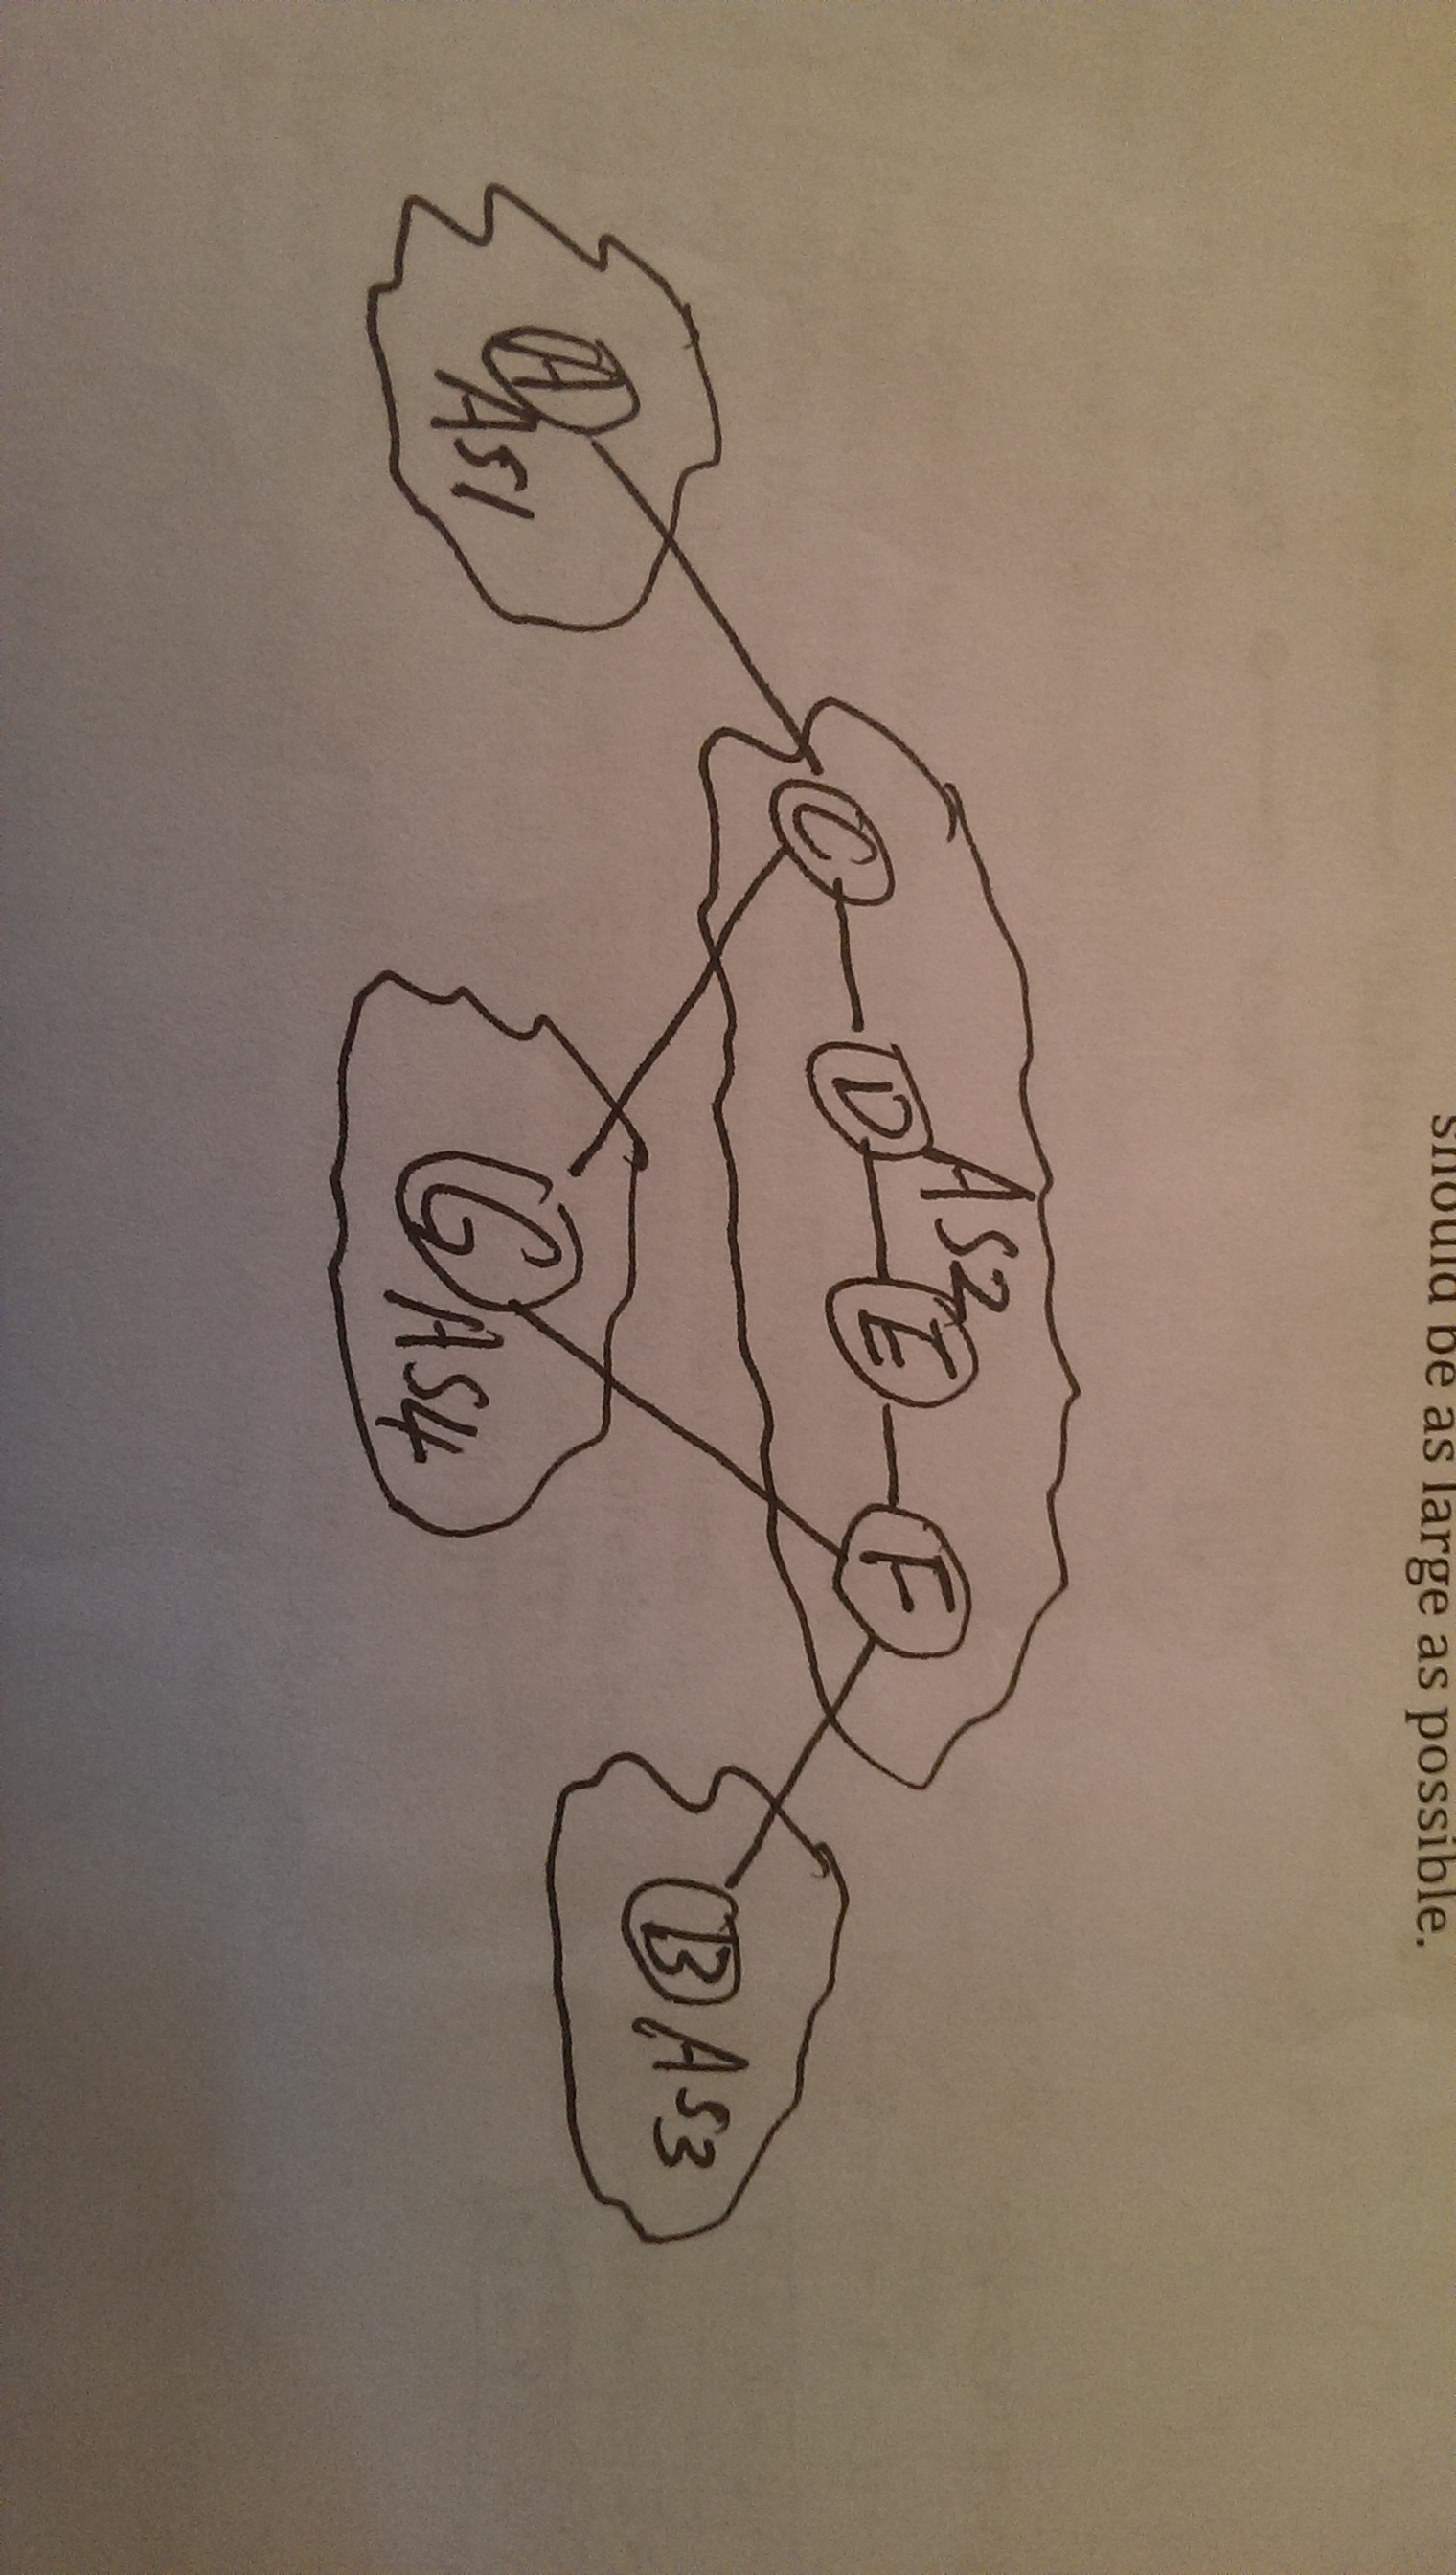
\includegraphics[scale=0.08,angle=90]{hw2.jpg}\\
The shortest path is A$\to$C$\to$G$\to$F$\to$B in terms of routers and 1$\to$2$\to$4$\to$2$\to$3 in terms of ASes.
\subsection*{(b)}
Because RIP will always choose the shortes path, RIP will choose A$\to$C$\to$G$\to$F$\to$B in terms of routers as the path from A to B.
\subsection*{(c)}
ForBGP, becaues it prefer the path with fewer ASes, BGP will choose A$\to$C$\to$D$\to$E$\to$F$\to$B in terms of routers as the path from A to B
\label{pg:end-of-p2}

%Insert solution here

% Make sure that the solution here does not exceed one page here. If
% it does, use the extra space for this problem at the end.  
%
% Comment out the next line if you are NOT using the extra space
%\paragraph{} \emph{Continued on Page \pageref{pg:p2-continuation}}



\newpage

\section*{Problem 3}
\subsection*{(a)}
Assume ACK size is negligible\\
160kbps*125ms/1kB=2.5
Because the size of window must be an integer, $W_S$=2
\subsection*{(b)}
Because we assume there is no proccessing time, every time receiver receive a packet it will immediately send a ACK back to sender. So $W_R=1$ is enough.
\subsection*{(c)}
For selective acknowledgement, because every time receiver receive a packet that is not in the right order, receiver do not drop it and store it in the buffer, send ACK for the packet back to sender. And send does not receive the ACK for the packet that should be in the right order, sender will resend a new one. Before receiver receives the new packet that is in the right order, it will just store all other packet that are not in order in buffer. So the maximum numer of packets receiver will store is equal to the size of sender. So we want $W_R=W_S$
\label{pg:end-of-p3}

% Make sure that the solution here does not exceed one page here. If
% it does, use the extra space for this problem at the end.  
%
% Comment out the next line if you are NOT using the extra space
%\paragraph{} \emph{Continued on Page \pageref{pg:p3-continuation}}




\newpage

\section*{Problem 4}
(c) and (e) are True
\label{pg:end-of-p4}

% Make sure that the solution here does not exceed one page here. If
% it does, use the extra space for this problem at the end.  
%
% Comment out the next line if you are NOT using the extra space
%\paragraph{} \emph{Continued on Page \pageref{pg:p4-continuation}}


\newpage

\section*{Problem 5}
\subsection*{(a)}
1-6 and 22-25
\subsection*{(b)}
6-14 and 15-21
\subsection*{(c)}
A triple duplicate ACK.
\subsection*{(d)}
32
\subsection*{(e)}
40/2=20
\subsection*{(f)}
24/2=12
\subsection*{(g)}
Assume the duplicate ACKs occures immediately before the end of $26^{th}$\\
CWND=8/2=4\\
SSTHRESH=12/2=6
\label{pg:end-of-p5}

%Insert solution here


% Make sure that the solution here does not exceed one page here. If
% it does, use the extra space for this problem at the end.  
%
% Comment out the next line if you are NOT using the extra space
%\paragraph{} \emph{Continued on Page \pageref{pg:p5-continuation}}


\newpage


\section*{Problem 6}

\subsection*{Part (a)}
Traceroute transmits packets with small Time To Live values; each time a packet pass through a router, Time To Live value decreaase by 1. When TTL value goes to zero the packet expire and traceroute sends back the information using ICMP Time Exceeded message back to sender.
\subsection*{Part (b)}
traceroute to 216.81.59.173 (216.81.59.173), 64 hops max, 52 byte packets\\
 1  * * *\\
 2  [AS25] xe-1-2-0-1985.inr-306-sut.berkeley.edu (136.152.20.1)  9.998 ms  4.052 ms  6.365 ms\\
 3  [AS25] t5-4.inr-202-reccev.berkeley.edu (128.32.0.58)  5.928 ms  4.119 ms  5.664 ms\\
 4  [AS25] xe-5-1-0.inr-001-sut.berkeley.edu (128.32.0.66)  10.423 ms  12.599 ms  48.544 ms\\
 5  [AS2152] cenic.net (137.164.50.16)  4.590 ms  4.064 ms  7.608 ms\\
 6  [AS2152] oak-agg2--sfo-agg1-10g.cenic.net (137.164.22.25)  8.006 ms  24.223 ms  28.060 ms\\
 7  [AS2152] dc-paix-px1--oak-core1-ge.cenic.net (137.164.47.18)  6.310 ms  6.945 ms  6.778 ms\\
 8  [AS2152] hurricane--paix-px1-ge.cenic.net (198.32.251.70)  11.935 ms  45.858 ms  16.560 ms\\
 9  [AS6939] 10gigabitethernet3-1.core1.sjc2.he.net (72.52.92.70)  27.641 ms  7.918 ms  52.378 ms\\
10  [AS6939] 10gigabitethernet14-7.core1.lax2.he.net (184.105.213.5)  15.071 ms  104.214 ms  22.345 ms\\
11  [AS46841] 10gigabitethernet2-3.core1.phx2.he.net (184.105.222.85)  31.365 ms  26.236 ms  25.737 ms\\
12  [AS46841] 10gigabitethernet5-3.core1.dal1.he.net (184.105.222.78)  55.314 ms  46.131 ms  46.376 ms\\
13  [AS6939] 10gigabitethernet5-4.core1.atl1.he.net (184.105.213.114)  87.504 ms  74.713 ms  78.964 ms\\
14  [AS6939] 216.66.0.26 (216.66.0.26)  67.796 ms  66.816 ms  66.943 ms\\
15  * * *\\
16  [AS21513] episode.iv (206.214.251.1)  117.155 ms  106.257 ms  108.214 ms\\
17  [AS21513] a.new.hope (206.214.251.6)  107.776 ms  108.208 ms  109.204 ms\\
18  [AS21513] it.is.a.period.of.civil.war (206.214.251.9)  108.309 ms  109.786 ms  109.637 ms\\
19  [AS21513] rebel.spaceships (206.214.251.14)  107.540 ms  107.145 ms  108.954 ms\\
20  [AS21513] striking.from.a.hidden.base (206.214.251.17)  109.116 ms  110.270 ms  106.703 ms\\
21  [AS21513] have.won.their.first.victory (206.214.251.22)  107.468 ms  106.741 ms  106.895 ms\\
22  [AS21513] against.the.evil.galactic.empire (206.214.251.25)  106.948 ms  108.344 ms  115.134 ms\\
23  [AS21513] during.the.battle (206.214.251.30)  107.989 ms  262.536 ms  108.244 ms\\
24  [AS21513] rebel.spies.managed (206.214.251.33)  106.811 ms  115.184 ms  106.614 ms\\
25  [AS21513] to.steal.secret.plans (206.214.251.38)  107.148 ms  108.845 ms  109.227 ms\\
26  [AS21513] to.the.empires.ultimate.weapon (206.214.251.41)  107.577 ms  110.484 ms  108.883 ms\\
27  [AS21513] the.death.star (206.214.251.46)  109.148 ms  108.671 ms  106.530 ms\\
28  [AS21513] an.armored.space.station (206.214.251.49)  106.450 ms  107.384 ms  106.645 ms\\
29  [AS21513] with.enough.power.to (206.214.251.54)  109.851 ms  108.454 ms  107.584 ms\\
30  [AS21513] destroy.an.entire.planet (206.214.251.57)  106.931 ms  132.208 ms  122.881 ms\\
31  [AS21513] pursued.by.the.empires (206.214.251.62)  107.421 ms  111.301 ms  117.747 ms\\
32  [AS21513] sinister.agents (206.214.251.65)  114.066 ms  107.710 ms  109.741 ms\\
33  [AS21513] princess.leia.races.home (206.214.251.70)  111.802 ms  381.459 ms  109.925 ms\\
34  [AS21513] aboard.her.starship (206.214.251.73)  108.241 ms  112.449 ms  111.891 ms\\
35  [AS21513] custodian.of.the.stolen.plans (206.214.251.78)  110.809 ms  107.928 ms  109.313 ms\\
36  [AS21513] that.can.save.her (206.214.251.81)  108.153 ms  108.956 ms  109.751 ms\\
37  [AS21513] people.and.restore (206.214.251.86)  108.020 ms  111.282 ms  107.646 ms\\
38  [AS21513] freedom.to.the.galaxy (206.214.251.89)  111.601 ms  112.989 ms  148.747 ms\\
39  [AS21513] 0-----i-------i-----0 (206.214.251.94)  171.349 ms  111.278 ms  255.688 ms\\
40  [AS21513] 0------------------0 (206.214.251.97)  111.147 ms  109.661 ms  110.565 ms\\
41  [AS21513] 0-----------------0 (206.214.251.102)  113.751 ms  109.153 ms  110.352 ms\\
42  [AS21513] 0----------------0 (206.214.251.105)  107.836 ms  110.324 ms  110.251 ms\\
43  [AS21513] 0---------------0 (206.214.251.110)  111.513 ms  108.142 ms  109.000 ms\\
44  [AS21513] 0--------------0 (206.214.251.113)  111.099 ms  108.126 ms  141.220 ms\\
45  [AS21513] 0-------------0 (206.214.251.118)  107.918 ms  108.408 ms  108.560 ms\\
46  [AS21513] 0------------0 (206.214.251.121)  107.929 ms  107.867 ms  111.001 ms\\
47  [AS21513] 0-----------0 (206.214.251.126)  111.123 ms  108.693 ms  110.930 ms\\
48  [AS21513] 0----------0 (206.214.251.129)  108.813 ms  132.312 ms  110.502 ms\\
49  [AS21513] 0---------0 (206.214.251.134)  112.031 ms  109.692 ms  111.276 ms\\
50  [AS21513] 0--------0 (206.214.251.137)  114.344 ms  281.457 ms  108.667 ms\\
51  [AS21513] 0-------0 (206.214.251.142)  107.841 ms  110.697 ms  108.941 ms\\
52  [AS21513] 0------0 (206.214.251.145)  109.620 ms  112.306 ms  115.584 ms\\
53  [AS21513] 0-----0 (206.214.251.150)  109.743 ms  109.469 ms  111.456 ms\\
54  [AS21513] 0----0 (206.214.251.153)  108.466 ms  113.609 ms  161.267 ms\\
55  [AS21513] 0---0 (206.214.251.158)  114.251 ms  223.281 ms  110.124 ms\\
56  [AS21513] 0--0 (206.214.251.161)  111.517 ms  110.879 ms  118.374 ms\\
57  [AS21513] 0-0 (206.214.251.166)  145.623 ms  115.682 ms  110.880 ms\\
58  [AS21513] 00 (206.214.251.169)  114.814 ms  109.668 ms  111.022 ms\\
59  [AS21513] i (206.214.251.174)  111.328 ms  109.265 ms  111.434 ms\\
60  [AS21513] by.ryan.werber (206.214.251.177)  114.727 ms  113.186 ms  112.014 ms\\
61  [AS21513] blizzards.breed.ccie.creativity (206.214.251.182)  108.757 ms  109.779 ms  111.208 ms\\
62  [AS21513] please.try.again.tracerote.to.obiwan.scrye.net (206.214.251.185)  109.795 ms  118.435 ms  110.403 ms\\
63  [AS21513] read.more.at.beaglenetworks.net (206.214.251.190)  116.403 ms *  122.843 ms\\
\subsection*{(c)}
$<$AS25,Berkeley$><$AS2152,Cenic$><$AS6939,He$><$AS46841,He$>$
\subsection*{(d)}
Cenic$\to$He
\subsection*{(e)}
It means the packet is not acknowledged within the expected timeout.\\
It may because of the newwork is busy and the packet was droped from the buffering queue.
\label{pg:end-of-p6}

% Make sure that the solution here does not exceed one page here. If
% it does, use the extra space for this problem at the end.  
%
% Comment out the next line if you are NOT using the extra space
%\paragraph{} \emph{Continued on Page \pageref{pg:p6-continuation}}


\newpage


%% Comment out the "extra spaces" completely for the problems for you
%% don't need them

%\section*{Extra space for Problem 1}
%\emph{Continued from Page \pageref{pg:end-of-p1}}\\

%Insert solution here


%\label{pg:p1-continuation}
%\newpage
%%Comment out the above three lines if you are not using extra space
%%for this problem.


%\section*{Extra space for Problem 2}
%\emph{Continued from Page \pageref{pg:end-of-p2}}\\

%Insert solution here

%\label{pg:p2-continuation}
%\newpage
%%Comment out the above three lines if you are not using extra space
%%for this problem.


%\section*{Extra space for Problem 3}
%\emph{Continued from Page \pageref{pg:end-of-p3}}\\

%Insert solution here

%\label{pg:p3-continuation}
%\newpage
%%Comment out the above three lines if you are not using extra space
%%for this problem.



%\section*{Extra space for Problem 4}
%\emph{Continued from Page \pageref{pg:end-of-p4}}\\

%Insert solution here

%\label{pg:p4-continuation}
%\newpage
%%Comment out the above three lines if you are not using extra space
%%for this problem.



%\section*{Extra space for Problem 5}
%\emph{Continued from Page \pageref{pg:end-of-p5}}\\

%Insert solution here


%\label{pg:p5-continuation}
%\newpage
%%Comment out the above three lines if you are not using extra space
%%for this problem.


%\section*{Extra space for Problem 6}
%\emph{Continued from Page \pageref{pg:end-of-p6}}\\


%Insert solution here


%\label{pg:p6-continuation}
%\newpage
%%Comment out the above three lines if you are not using extra space
%%for this problem.



\end{document}